\chapter{Aberration Correction for Spinning Disk Confocal Microscopy}
\label{chpt:Aurox}

\section{Aberrations and Image Formation}
\label{subsec:Aurox_aberrations}

Section~\ref{sec:aberrations} has already discussed the origin of 
optical aberrations and their effect on image formation for 
conventional imaging techniques. Such effects are still relevant
and degrade the image quality in the Aurox Clarity system. In addition,
in the excitation path aberrations have the effect of blurring the 
disk image on the sample which results in a loss of contrast and 
axial resolution due to reduction in spatial frequency
information\cite{wilson1990confocal, hell1993aberrations}. In the 
emission path, the fluorescence signal of the sample is similarly
degraded leading to a reduction of the signal in both $I_{T}$ and
$I_{R}$, hence a reduction in the SNR of $I_{conf}$. 

\section{Biological Exemplar}
\label{sec:Aurox_biology}

To demonstrate the improvement in image quality adaptive optics
provides in the Aurox Clarity system, we utilise two samples from
\textit{Drosophila melanogaster}; neuro-muscular junctions, NMJ, 
and egg chambers.

\subsection{Sample preparation}
\label{subsec:Aurox_sample_prep}

\subsubsection{Neuro-muscular Junction}
\label{subsubsec:Aurox_NMJ_prep}

The \textit{Drosophila melanogaster} neuro-muscular junction (NMJ) 
samples were prepared by following the protocol. 
3rd instar \textit{Drosophila melanogaster} larvae (Oregon-R 
strain) were dissected in HL3 buffer with $0.3mM~\text{Ca}^{2+}$ to 
prepare a larval fillet. After this, larvae were fixed with 
4\% paraformaldehyde and blocked using 1\% BSA.\cite{brent2009drosophila} Larvae were stained overnight with 1:100 Horseradish Peroxidase (HRP) 
conjugated to Alexa568 fluorophore to visualise the neurons, and 
primary mouse antibody against Discs large (DLG) to visualise the 
postsynaptic density. The next day, the larvae were counterstained 
with secondary antibody to detect the DLG (1:200 donkey anti-mouse 
conjugated to Alexa488 fluorophore was used), as well as 1:1000 from 1mg/mL 
stock DAPI to visualise the nuclei. The larvae were then washed and mounted 
in 65\% vectashield\cite{brent2009drosophila}. This dilution of 
vectashield is compatible with the AMEP4694 $60\times$, 1.42 NA oil 
immersion lens.

\subsubsection{Egg chambers}
\label{subsubsec:Aurox_Egg_chambers_prep}


The \textit{Drosophila melanogaster} egg chamber samples were prepared by the 
following protocol. Ovaries were isolated from \textit{Drosophila 
melanogaster} adult females straight into fixation medium and fixed in 4\% PFA 
(prepared fresh from a stock solution of 16\% paraformaldehyde, methanol free 
ultra - pure EM grade, Polysciences) in Cytoskeleton Buffer for 10 minutes 
without added 
detergent\cite{jia2016automatic,zhang2020nanoscale,leyton2016pfa}.  Ovaries 
were then heptane permeabilised with 800$\mu$l heptane and post fixed in 4\% 
PFA in PBS for not more than 15 minutes, then washed three times with 
PBS/TX-100, 0.05\%. Actin was labelled with phalloidin Alexa 488 Phalloidin: 
stock 200 units/ml in Methanol, 6.6 $\mu$M) at between 5 and 20 $\mu$l stock 
in 200 $\mu$l for at least 45 min at RT (or O/N at $4^{\circ}$C). Labelled 
ovarioles were washed three times with PBS TX-100, 0.05\%, and then finally 
with PBS before being pre-incubated at RT for at least 3 hours in 70\% 
Vectashield. This was removed and replaced with fresh 70\% Vectashield prior 
to samples being mounted under a coverslip raised on two thin strips of 
double-sided sticky tape to avoid flattening\cite{davidson2016localized}. The 
edges of the coverslips were double varnished, and slides were stored at 
$4^{\circ}$C until use.

\section{Experimental Results}
\label{sec:Aurox_results}

The same aberration modes were corrected for all the results presented. 
These are oblique and vertical astigmatism, vertical and horizontal coma 
and primary spherical, corresponding to Noll indices 5, 6, 7, 8 and 11 
respectively\cite{noll1976zernike}. These are the low order optical 
aberrations whose effects are particularly detrimental to image quality. For example, 
spherical aberration has been shown to reduce peak intensity by 40\% at
a focal plane 20$\mu$m deep compared to a focal plane 10$\mu$m 
deep\cite{hell1993aberrations}. To show the effectiveness of aberration 
correction throughout the sample, the sensorless adaptive optics correction
routine described in Section~\ref{subsec:sensorless_correction} was performed
at multiple depths in the neuro-muscular junction samples. Figure~\ref{fig:Aurox_depth_comparison_composite} shows the results of 
these corrections. At all imaging depths, aberration correction yields an 
improvement in both contrast and overall image intensity. This improvement 
in image quality reveals biological structures which, without correction, 
are not visible. Overall intensity does decrease with imaging depth likely 
due to a combination of varying marker density throughout the sample, 
residual aberration and loss of signal through absorption or scattering 
as the light passes through more tissue.

\begin{figure}[h]
	\centering
	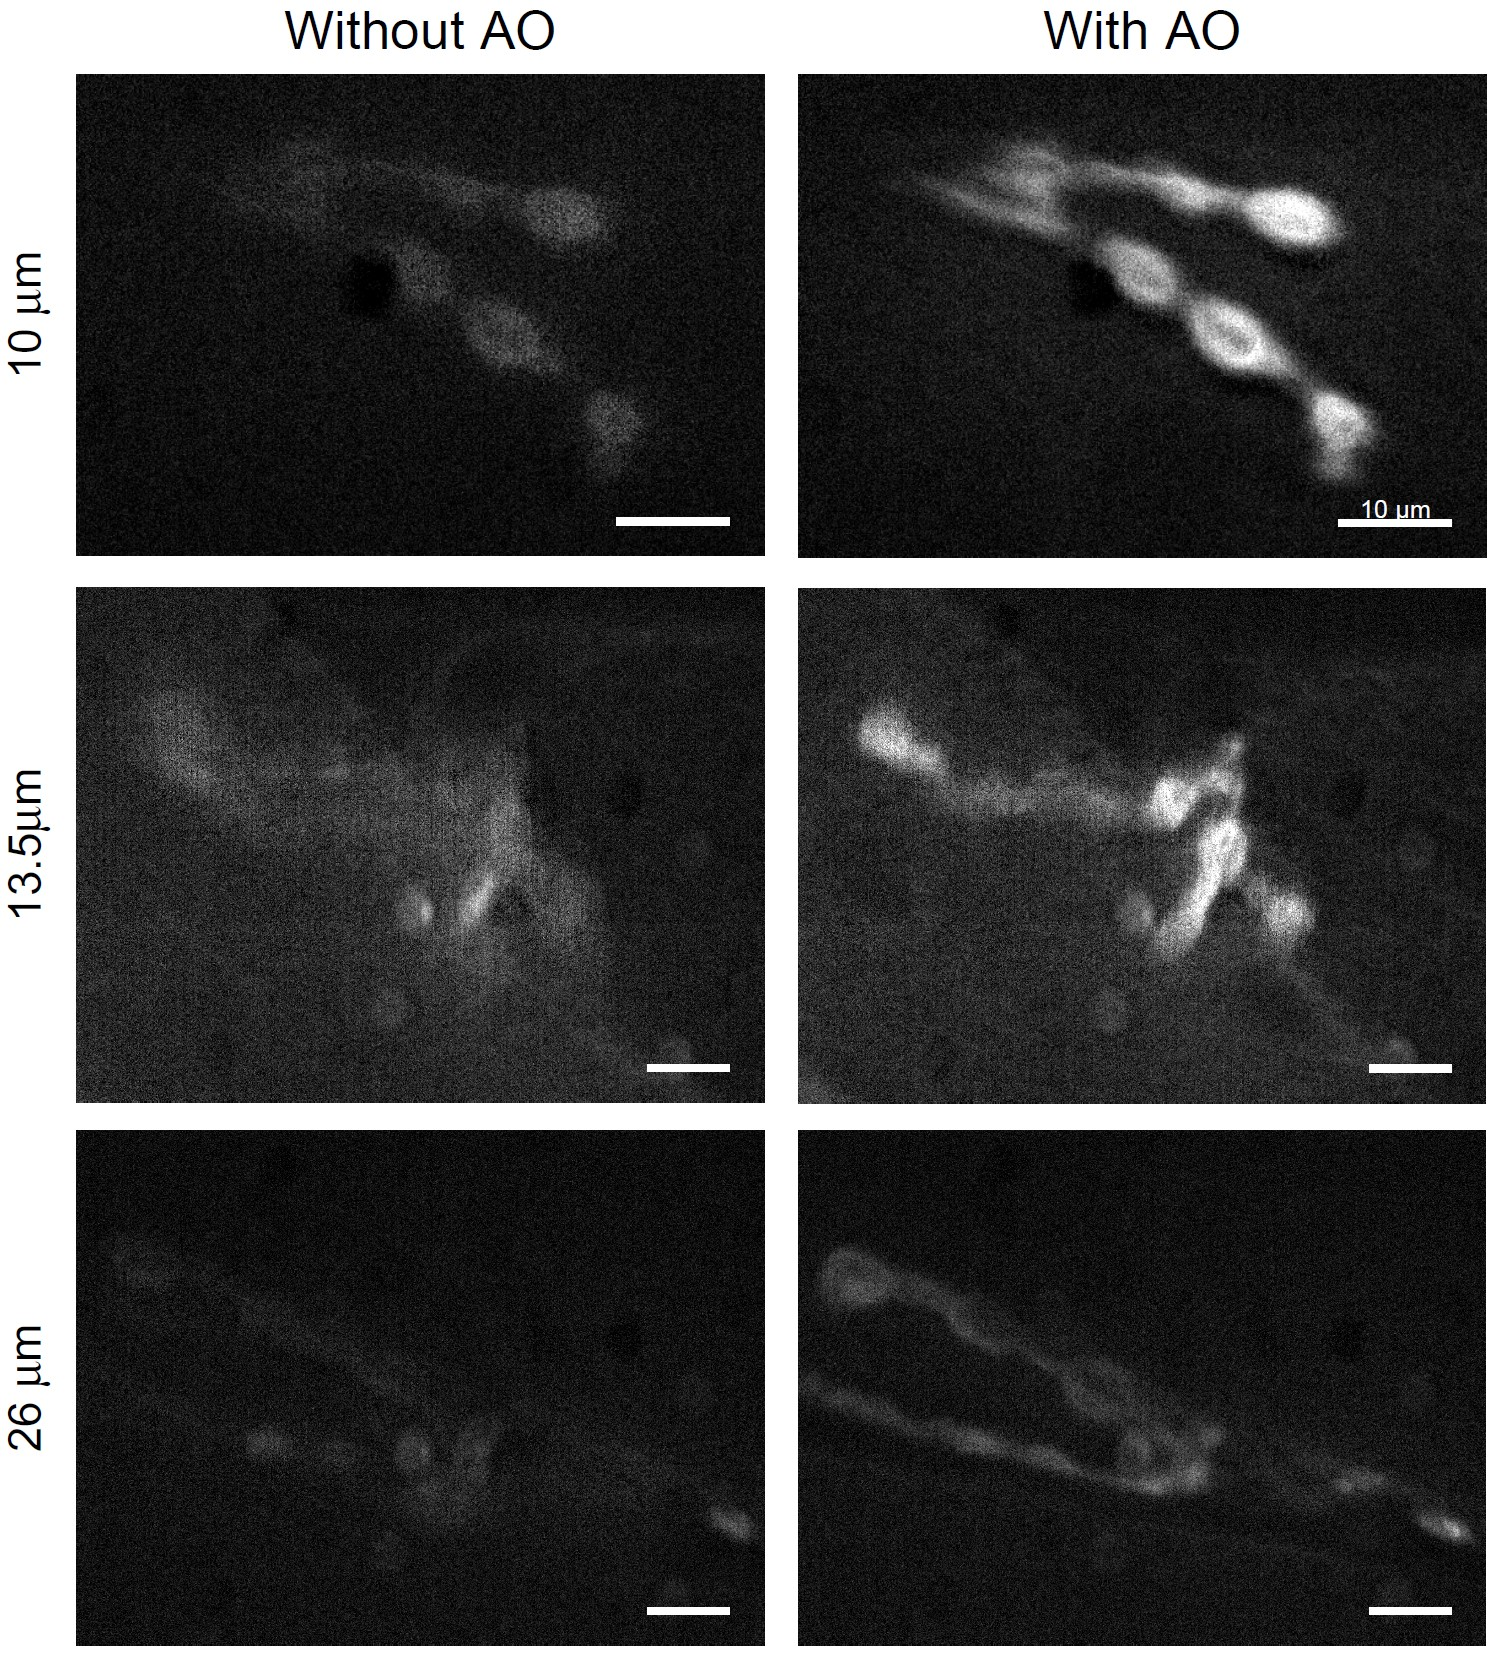
\includegraphics[width=\textwidth]{images/Aurox_depth_comparison_composite.jpg}
	\caption[Depth comparison of the Aurox imaging system]{Neuro-muscular 
		junction images acquired at 10$\mu$m, 13.5$\mu$m and 26$\mu$m with 
		high optical sectioning. The images are of single Z-positions. 
		Aberration correction yields improvements in signal and contrast 
		at all depths. Scale bars are all 10$\mu$m. Discs large (DLG) 
		counterstained with secondary antibody to detect the DLG (donkey 
		anti-mouse conjugated to Alexa 488 fluorophore) is shown. 
		All images are displayed on the same intensity scale.}
	\label{fig:Aurox_depth_comparison_composite}
\end{figure}

Since the egg chambers samples were fixed and cleared, the sample induced 
aberrations were considerably less severe over a larger Z range. 
Figure~\ref{fig:Aurox_egg_chambers_composite} shows maximum intensity 
projections of 36$\mu$m Z-stacks obtained at high optical sectioning, both
without and with aberration correction. Ovarioles were separated out to 
better visualise individual egg-chambers Once again the overall contrast 
and intensity are improved with aberration correction. This is most 
noticeable with the actin associated with ring-canals. Ring-canals are pores 
which connect the oocyte to adjacent nurse cells, which supports oocyte 
growth\cite{loyer2015drosophila}. In many of the cases highlighted in 
Figure~\ref{fig:Aurox_egg_chambers_composite} with the arrows, the ring 
structure of these ring-canals is not visible without aberration correction.

\begin{figure}[h]
	\centering
	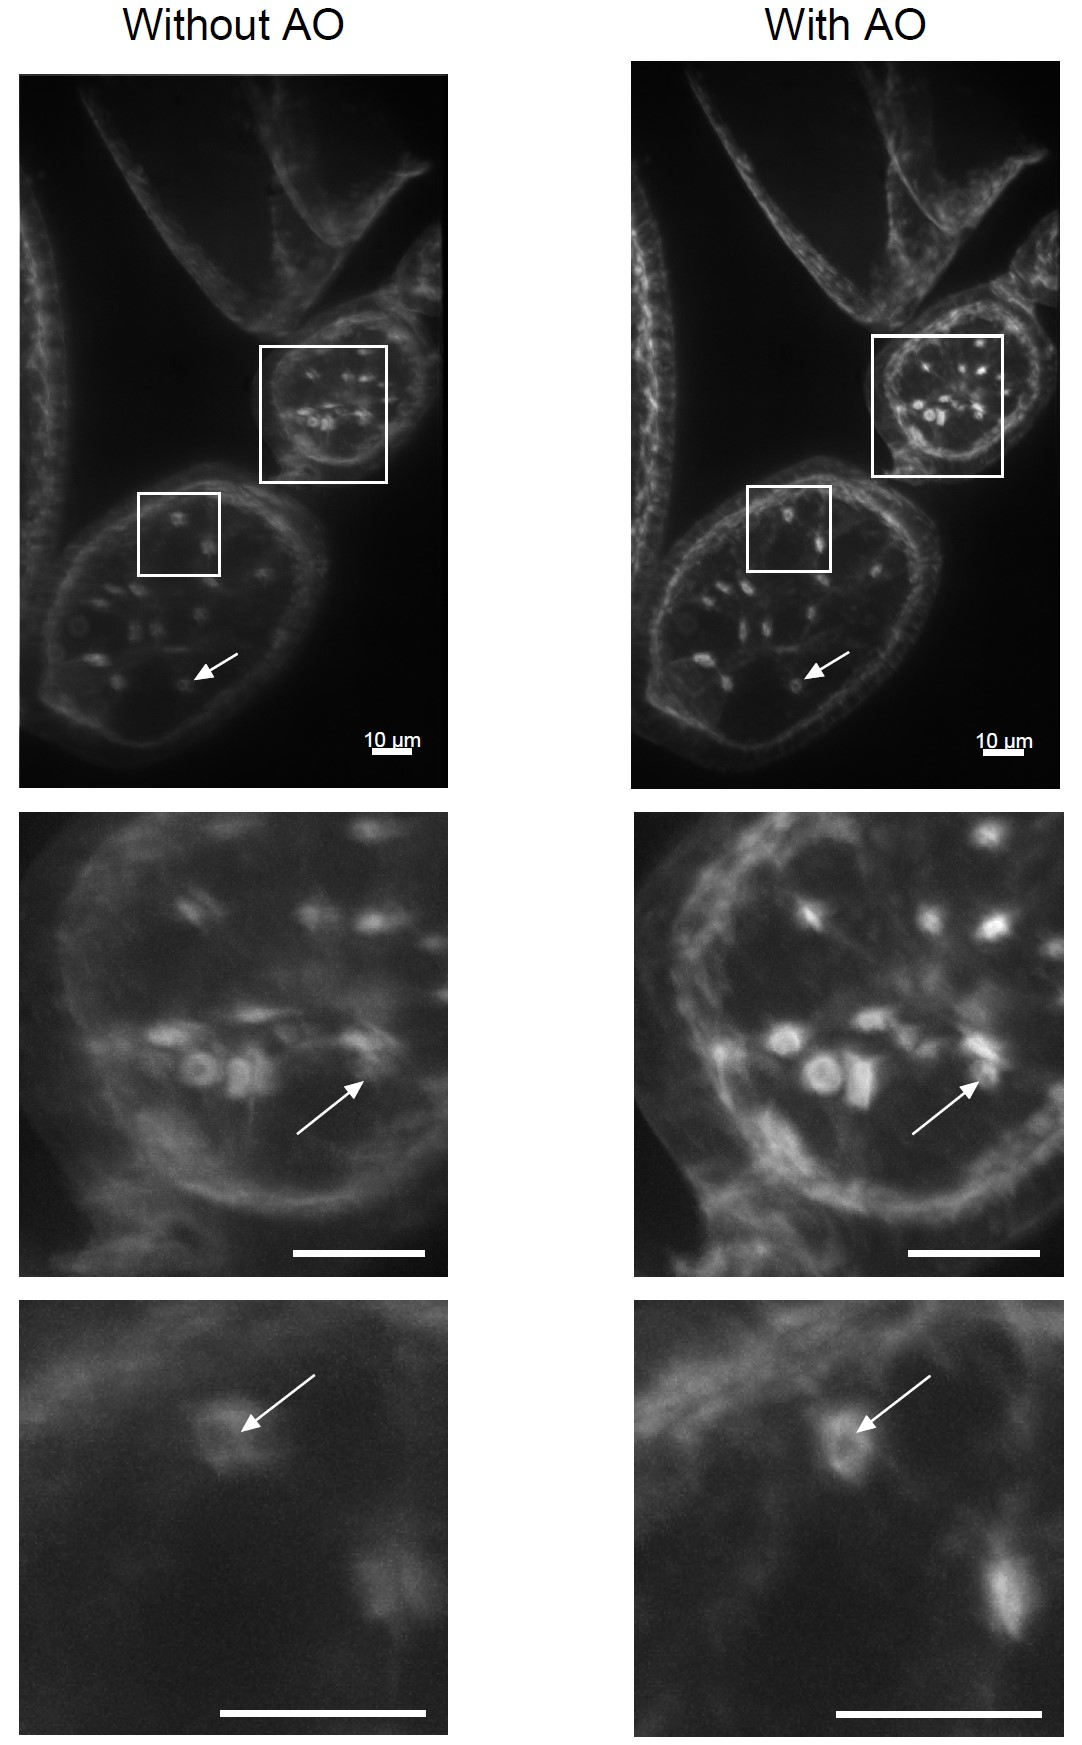
\includegraphics[width=0.8\textwidth]{images/Aurox_egg_chambers_composite.jpg}
	\caption[\textit{Drosophila} egg chamber data acquired on the Aurox imaging 
	system]{Maximum intensity projections of 36$\mu$m Z-stacks of egg 
		chamber samples acquired without (left) and with (right) adaptive 
		optics correction at high optical sectioning. The overall intensity 
		and contrast are improved after correction. The arrows highlight 
		particularly notable areas of improvement where fine details, such 
		as the outline of ring canals, become clearly visible. Scale bars 
		are all 10$\mu$m. Actin (labelled with phalloidin Alexa 488) signal 
		is shown. All images are displayed on the same intensity scale.}
	\label{fig:Aurox_egg_chambers_composite}
\end{figure}

Finally, Figure~\ref{fig:Aurox_NMJ_composite_grey_and_color} shows maximum 
intensity projections of 20$\mu$m Z-stacks obtained at high optical 
sectioning, both without and with aberration correction. Despite the 
sensorless adaptive optics routine being performed only using the data 
from the Alexa568 (HRP) channel, improvements in intensity and contrast
are observed in all imaging channels. Notably, the aberration correction 
allows for individual fibres in the segmental nerve to be resolved, shown in 
the middle row of Figure~\ref{fig:Aurox_NMJ_composite_grey_and_color}. Without
aberration correction the structure of individual round postsynaptic 
densities, boutons, are either unclear or not visible, shown in the bottom 
row of Figure~\ref{fig:Aurox_NMJ_composite_grey_and_color}. Once the sample 
induced aberrations have been corrected, the structure of these boutons 
becomes clearer and the presence of several new, previously obscured, boutons 
can be observed.

\begin{figure}[h]
	\centering
	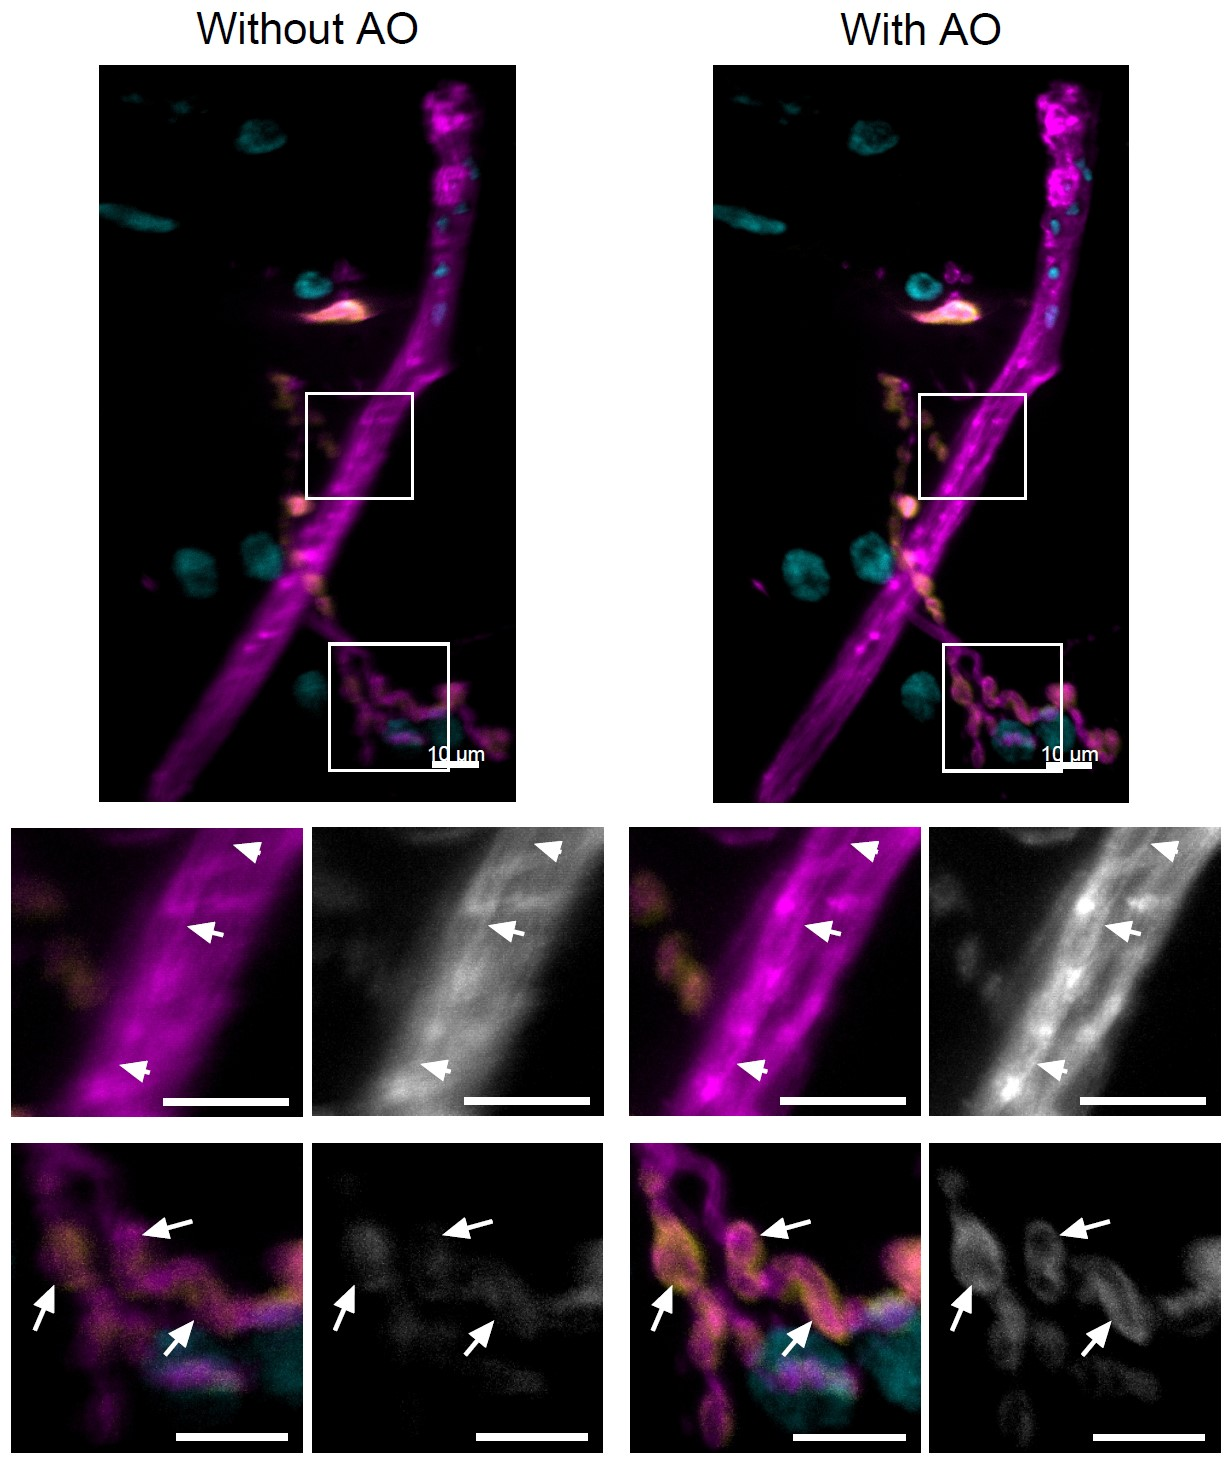
\includegraphics[width=\textwidth]{images/Aurox_NMJ_composite_grey_and_color.jpg}
	\caption[\textit{Drosophila} neuro-muscular junction data acquired on the Aurox imaging 
	system]{Maximum intensity projections of 20$\mu$m $z$-stacks of 
		neuro-muscular junction samples acquired without (left) and with 
		(right) AO correction at high optical sectioning. Discs large (DLG) 
		counterstained with secondary antibody to detect the DLG (donkey 
		anti-mouse conjugated to Alexa 488 fluorophore) is shown in 
		yellow. Horseradish Peroxidase (HRP) (conjugated to Alexa 568 
		fluorophore) to visualise the neurons is shown in magenta, nuclei 
		shown in cyan. Middle row greyscale images show only HRP. Bottom row 
		greyscale images show only DLG. The overall intensity and contrast 
		are improved after correction. The arrows highlight particularly 
		notable areas of improvement where fine details, such as individual 
		nerve fibres, become clearly visible. Scale bars are all 10$\mu$m. 
		All images are displayed on the same intensity scale.}
	\label{fig:Aurox_NMJ_composite_grey_and_color}
\end{figure}
